% ProjectD

\chapter{Project Description}

\label{ProjectD}

\lhead{Chapter 5. \emph{Project Description}}

%----------------------------------------------------------------------------------------
%	Ara platform discovery
%----------------------------------------------------------------------------------------

\section{Ara platform study}

In this section, we will describe different studies and preliminary experimentation we've done before designing  the module.

In fact, because of the lake of literature or past experience with the Ara platform, we first need to study the Ara Module Development Kit send by Google ATAP. We focus on understanding the role of each board, and there I/O - regarding protocols and speed. Then we determine the reliable rate on witch the operating system can execute a single task - such as I/O operation. Finally we perform some benchmark and CPU load test. 

\subsection{MDK and boards study}



\subsection{Android for ARA reliable I/O operation rate}  \label{result-ara}


\subsubsection{Problematic}

In this part, we would determine the I/O performance between the Ara main board and  modules in order to fit its characteristics: maximum DAC sampling rate, resolution, buffering needs.

We focused on the minimum stable thread execution speed, which fix the number of Android I/O operation per second, then the maximum number of bytes we can read each time.

\subsubsection{Protocol}
We modify the oxymeter application changing the thread execution interval from 1ms to 100ms and record the effective execution period using time-stamps. To have a set consistent datasets, we record 1 million of sample for each measure. As consequence, we would be able to determine the minimum thread execution period, and its stability.
This point is particularly important for designing the buffer on the VLC receiver : a bigger I/O operation period than expected will cause overflow, and data loss of data.

To determine the bus speed and the max effective transferred without error for each operation, we replaced the oxymeter module by an Arduino that will write diferents among of data on the bus. In addition, we use a logic analyzer to record what's happening on the bus.

\subsubsection{Results}
\begin{itemize}

\begin{figure}[h]
  \begin{minipage}[c]{.46\linewidth}
    \centering
    \scalebox{1}{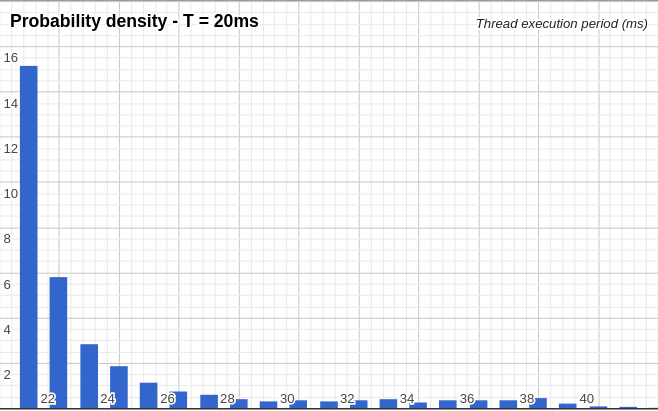
\includegraphics[width=\textwidth]{Pictures/dsp20.png}}
    \label{fig:dsp20}
    \rule{16em}{0.5pt}
    \caption[Waveform on power-linel]{Waveform on power-line}
  \end{minipage}
  \hfill%
  \begin{minipage}[c]{.46\linewidth}
  \centering
    \scalebox{1}{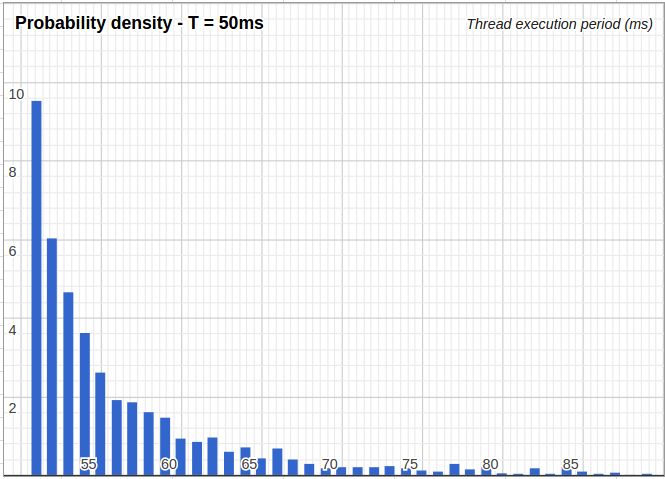
\includegraphics[width=\textwidth]{Pictures/dsp50.png}}
    \label{fig:dsp50}
    \rule{16em}{0.5pt}
    \caption[Waveform on power-linel]{Waveform on power-line}
  \end{minipage}
\end{figure}

\item Android threads can't reach lower period than 8ms but with an elevate variance, as we can see in .

\item Performing statistical analysis, for each execution period and plotting the effective period distribution and variance, we can consider 30ms as safe.

\item Even if the I2C bus speed clock should be 400kHz - according to the Ara MDK documentation - the effective clock rate is 133kHz.
On other hand, even if the kernel driver limits I/O operations to 512 bytes, the bus gets corrupted trying to transfer more than 350 bytes per operation.
\end{itemize}

\subsubsection{Conclusion}  \label{conclusion-ara}
According to , we should design our VLC receiver module to taking account an effective bit-rate of 92,4 kbps and will developed the Android application with a module polling thread period to 30ms and an I2C transaction . 


\subsection{Ara benchmark}

In addition to \ref{result-ara}, we should be sure that a normal to extensive modular smartphone won't affect VLC module performances, even if the app run in background mode. In this case, the Android CPU governor will reduce the priority of our app, giving it less resources or stopping it if necessary.

In order to do that, we use a benchmark application that would simulate typical smartphone use-case : web browsing, shot-message writing, video playing or games.

During the stress tests, both CPU load and repartitions over running process, and RAM usage are monitored.

\begin{figure}[h]
  \begin{minipage}[c]{.46\linewidth}
    \centering
    \scalebox{0.9}{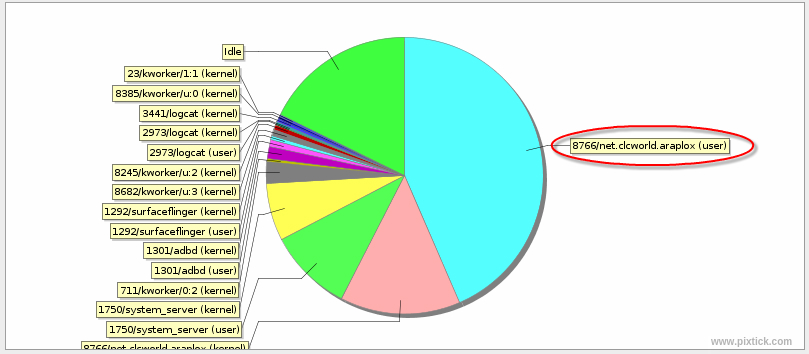
\includegraphics[width=\textwidth]{Pictures/cpu-singleapp.jpg}}
    \label{fig:cpu-single}
    \rule{16em}{0.5pt}
    \caption[Waveform on power-linel]{Waveform on power-line}
  \end{minipage}
  \hfill%
  \begin{minipage}[c]{.46\linewidth}
  \centering
    \scalebox{0.9}{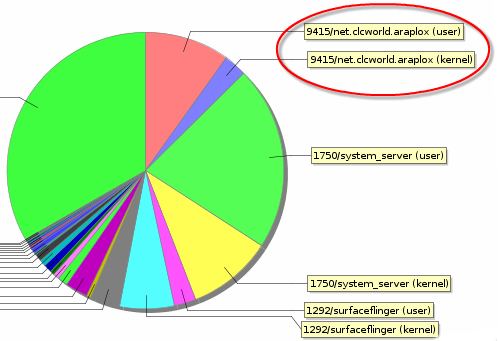
\includegraphics[width=\textwidth]{Pictures/cpu-loadapp.jpg}}
    \label{fig:cpu-load}
    \rule{16em}{0.5pt}
    \caption[Waveform on power-linel]{Waveform on power-line}
  \end{minipage}
\end{figure}

For each case, except the video game that made freeze and crash the Ara platform, results where exactly the same than with a single activity - ie. just our application - and we achieve the same bit-rate.

\subsubsection{Conclusion}


%----------------------------------------------------------------------------------------
%	Receiver circuit design
%----------------------------------------------------------------------------------------

\section{Receiver circuit design}

\subsection{Needs description}
\subsection{Photodiode}
\subsection{1st AOP : Current to tension converter}
\subsection{2sd: Low Pass filter}
\subsection{Gain}

%----------------------------------------------------------------------------------------
%	Emitter driver
%----------------------------------------------------------------------------------------

\section{Emitter driver}

\subsection{OOK modulation}
\subsection{4B6B Line coding}
\subsection{Algorithm}


%----------------------------------------------------------------------------------------
%	Receiver CAN and Buffer
%----------------------------------------------------------------------------------------

\section{Receiver CAN and Buffer}

\subsection{Digitalization}
\subsection{Decoding}
\subsection{Buffering}
\subsection{Input/output}

%----------------------------------------------------------------------------------------
%	Ara Android App
%----------------------------------------------------------------------------------------

\section{Ara Android App}

In this part, we describe the Android application that we have developed, to support our VLC receiver module.

\subsection{Application structure and operations}
Our application as been developed used Google Android API 18, to be compliant with the operating system version which has been installed on the AP Board.

The application package has been called respecting Java name convention : edu.upc.entel.wng.vlcAraModule and content 3 classes :

\begin{itemize}
\item VLCAraActivity : initialize the application and user interface. It surcharges the Activity class , as requested by the Android API.
\item Sensor : define and perform operations to communicate with our module such as I2C bus initialization, data polling as well as handling and message with the User Interface (UI).
\item VlcLogger : this class realize logging operation saving received data on the board internal storage or an external SD Card.
\end{itemize}

Application workflow is quiet simple :
\begin{enumerate}
\item Initialize and start the application main Activity.
\item Setup the I2C Bus.
\item Initialize the logger and create a log file.
\item Start the \textbf{Sensor} thread that poll I2C bus at defined interval and send the result to the android activity. 
\item Handle Sensor thread messaging and user interaction.
\end{enumerate}

\subsection{User Interface}

The application user interface as few components as defined in the XML activity layout description file :
\begin{itemize}
\item EditText field: used to display received bits.
\item "Clear" and "Save" Button :
\end{itemize}

Each component are placed in a horizontal layout container.

\subsection{I2C JNI interface}

As the Android Java API for the Ara Module Development Kit is the same as the standard API, we need to implement additional components in order to access the low level hardware such as the GPIO or the I2C bus.
The Ara MDK is provided with an operating system level driver, developed in C, that can be used to configure, read and write date, in a simple way.
However, this C interface, can't be directly used through the Java API. In order to give the possibility to perform I2C operations in our Android application, we develop a JNI interface that would wrap the C driver into a Java package.
So we define 2 Java classes : 
\begin{itemize}
\item I2CManager : it configures the i2c bus, by using UNIX I2C kernel driver and execute I2CTransaction.
\item I2CTransaction : it represents read or write operation on the bus.
\end{itemize}

Class methods are detailed in the Anexxe.

\subsection{Results}
\subsection{Interpretation}